% ============================================================
%  L02_mini10.tex  --  Fintech Ecosystem
%  10-Slide Arc: WHY > FEEL > WHAT > CASE > HOW > RISK > WHERE > IMPACT > SO WHAT > ACT
%  Self-contained (no \input{} commands, no \includegraphics)
%  Compile: pdflatex L02_mini10.tex  (twice for overlays)
% ============================================================

\documentclass[aspectratio=169, 11pt]{beamer}
\usetheme{Madrid}
\usecolortheme{whale}
\usepackage{tikz,pgfplots,booktabs,multicol,amsmath}
\usetikzlibrary{arrows.meta,positioning,shapes.geometric,calc,decorations.pathmorphing}
\pgfplotsset{compat=1.18}

% ---- Colour palette ----------------------------------------
\definecolor{mlpurple}{HTML}{9467BD}
\definecolor{mlblue}{HTML}{1F77B4}
\definecolor{mlred}{HTML}{D62728}
\definecolor{mlorange}{HTML}{FF7F0E}
\definecolor{mlgreen}{HTML}{2CA02C}
\definecolor{mlgray}{HTML}{7F7F7F}
\definecolor{mlteal}{HTML}{0D7377}
\definecolor{mlcyan}{HTML}{14BDEB}

% ---- Beamer theme overrides --------------------------------
\setbeamercolor{structure}{fg=mlteal}
\setbeamercolor{palette primary}{bg=mlteal,fg=white}
\setbeamercolor{palette secondary}{bg=mlteal!80,fg=white}
\setbeamercolor{palette tertiary}{bg=mlteal!60,fg=white}
\setbeamercolor{palette quaternary}{bg=mlteal,fg=white}
\setbeamercolor{frametitle}{bg=mlteal!10,fg=mlteal}
\setbeamercolor{title}{fg=white}
\setbeamercolor{subtitle}{fg=mlcyan}
\setbeamercolor{block title}{bg=mlteal,fg=white}
\setbeamercolor{block body}{bg=mlteal!8,fg=black}
\setbeamercolor{block title alerted}{bg=mlred,fg=white}
\setbeamercolor{block body alerted}{bg=mlred!8,fg=black}
\setbeamercolor{block title example}{bg=mlgreen,fg=white}
\setbeamercolor{block body example}{bg=mlgreen!8,fg=black}
\setbeamerfont{frametitle}{size=\large,series=\bfseries}

% ---- Bottom note command -----------------------------------
\newcommand{\bottomnote}[1]{%
  \vfill
  \begin{beamercolorbox}[wd=\textwidth,ht=2ex,dp=1ex]{palette primary}
    \tiny\hspace{1em}#1
  \end{beamercolorbox}}

% ---- Metadata ----------------------------------------------
\title{Fintech Ecosystem}
\subtitle{10-Slide Mini Lecture}
\author{Joerg Osterrieder}
\institute{University of Zurich}
\date{Spring 2026}
\setbeamertemplate{navigation symbols}{}

% ============================================================
\begin{document}
% ============================================================

% TITLE FRAME (not counted in the 10)
\begin{frame}
  \titlepage
\end{frame}

% ============================================================
%  FRAME 1 -- WHY: TikZ comic (farmer with mobile phone, closed bank)
% ============================================================
\begin{frame}{Why the Ecosystem Matters: The Unbanked Farmer}
\begin{center}
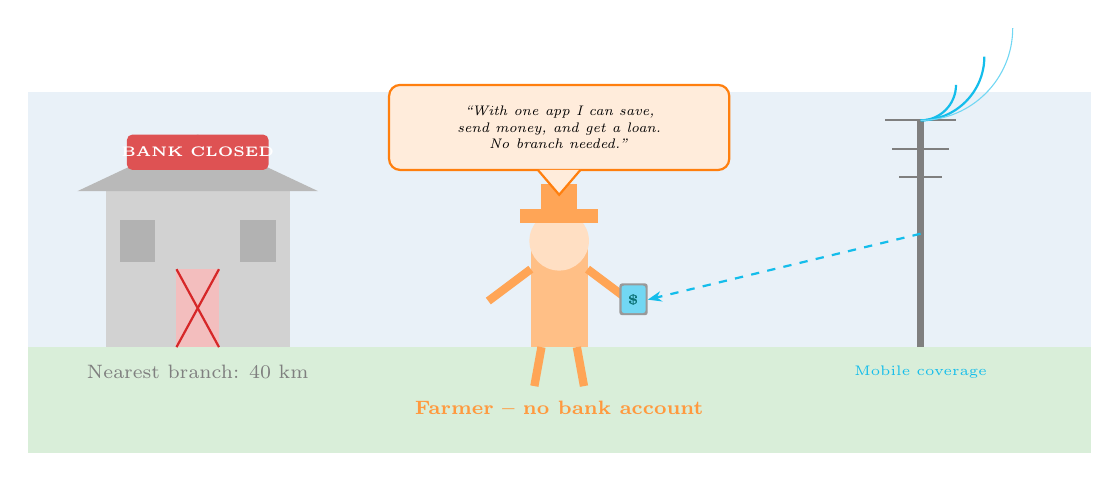
\begin{tikzpicture}[scale=0.90]

  % ---- Rural background: ground and sky ---------------------
  \fill[mlgreen!18] (-7.5,-1.5) rectangle (7.5,0.0);
  \fill[mlblue!10]  (-7.5, 0.0) rectangle (7.5,3.6);

  % ---- Closed bank branch (left side) ----------------------
  % Building body
  \fill[mlgray!35] (-6.4,0.0) rectangle (-3.8,2.2);
  % Roof
  \fill[mlgray!55] (-6.8,2.2) -- (-5.1,3.0) -- (-3.4,2.2) -- cycle;
  % Door (closed, with X)
  \fill[mlred!30] (-5.4,0.0) rectangle (-4.8,1.1);
  \draw[mlred,thick] (-5.4,0.0) -- (-4.8,1.1);
  \draw[mlred,thick] (-4.8,0.0) -- (-5.4,1.1);
  % Windows (shuttered)
  \fill[mlgray!60] (-6.2,1.2) rectangle (-5.7,1.8);
  \fill[mlgray!60] (-4.5,1.2) rectangle (-4.0,1.8);
  % Sign
  \fill[mlred!80,rounded corners=2pt] (-6.1,2.5) rectangle (-4.1,3.0);
  \node[font=\tiny\bfseries,text=white] at (-5.1,2.75) {BANK CLOSED};
  % Label
  \node[font=\scriptsize,text=mlgray] at (-5.1,-0.35) {Nearest branch: 40 km};

  % ---- Farmer figure (centre) ------------------------------
  % Body
  \fill[mlorange!50] (-0.4,0.0) rectangle (0.4,1.5);
  % Head
  \fill[mlorange!25] (0.0,1.5) circle (0.42);
  % Hat (simple wide-brim)
  \fill[mlorange!70] (-0.55,1.75) rectangle (0.55,1.95);
  \fill[mlorange!70] (-0.25,1.95) rectangle (0.25,2.30);
  % Arms
  \draw[mlorange!70,line width=3pt] (-0.4,1.1) -- (-1.0,0.65);
  \draw[mlorange!70,line width=3pt] ( 0.4,1.1) -- ( 1.0,0.65);
  % Legs
  \draw[mlorange!70,line width=3pt] (-0.25,0.0) -- (-0.35,-0.55);
  \draw[mlorange!70,line width=3pt] ( 0.25,0.0) -- ( 0.35,-0.55);
  % Phone in right hand
  \fill[mlgray!80,rounded corners=1pt] (0.85,0.45) rectangle (1.25,0.90);
  \fill[mlcyan!60,rounded corners=1pt] (0.88,0.48) rectangle (1.22,0.87);
  \node[font=\tiny\bfseries,text=mlteal] at (1.05,0.67) {\$};
  % Label
  \node[font=\scriptsize\bfseries,text=mlorange!80] at (0.0,-0.85)
    {Farmer -- no bank account};

  % ---- Farmer speech bubble --------------------------------
  \fill[mlorange!15,rounded corners=4pt] (-2.4,2.5) rectangle (2.4,3.7);
  \draw[mlorange,thick,rounded corners=4pt] (-2.4,2.5) rectangle (2.4,3.7);
  \fill[mlorange!15] (-0.3,2.5) -- (0.0,2.15) -- (0.3,2.5) -- cycle;
  \draw[mlorange,thick] (-0.3,2.5) -- (0.0,2.15) -- (0.3,2.5);
  \node[font=\tiny,text width=4.5cm,align=center] at (0.0,3.1)
    {\textit{``With one app I can save,}\\
     \textit{send money, and get a loan.}\\
     \textit{No branch needed."}};

  % ---- Mobile tower (right side) ---------------------------
  % Tower pole
  \draw[mlgray,line width=2.5pt] (5.1,0.0) -- (5.1,3.2);
  % Antenna cross-bars
  \draw[mlgray,thick] (4.6,3.2) -- (5.6,3.2);
  \draw[mlgray,thick] (4.7,2.8) -- (5.5,2.8);
  \draw[mlgray,thick] (4.8,2.4) -- (5.4,2.4);
  % Signal arcs
  \draw[mlcyan,thick] (5.1,3.2) arc(270:360:0.5);
  \draw[mlcyan,thick] (5.1,3.2) arc(270:360:0.9);
  \draw[mlcyan!60,thin] (5.1,3.2) arc(270:360:1.3);
  \node[font=\tiny,text=mlcyan] at (5.1,-0.35) {Mobile coverage};

  % ---- Arrow: tower to phone --------------------------------
  \draw[mlcyan,-{Stealth[length=5pt]},thick,dashed]
    (5.1,1.6) -- (1.25,0.67);

\end{tikzpicture}
\end{center}
\bottomnote{1.4 billion adults remain unbanked globally (World Bank 2023) -- yet two-thirds own a mobile phone. The ecosystem exists to close this gap.}
\end{frame}

% ============================================================
%  FRAME 2 -- FEEL: Text-only prompt (nudge exercise)
% ============================================================
\begin{frame}{A Nudge You Didn't Notice}

\vspace{0.2em}
\begin{block}{The Invisible Architecture of Your Banking App}
\small Every time you open your bank or fintech app, choices have already been made \emph{for} you.
Which account is shown first? What action is highlighted in green? What does the default saving rate say?
\end{block}

\vspace{0.2em}
\small Open your banking or payments app \emph{right now}. Look for:

\vspace{0.1em}
\begin{columns}[T]
\begin{column}{0.48\textwidth}
\begin{itemize}\small
  \item[\textcolor{mlteal}{\textbullet}] \textbf{A default} -- pre-filled amount, pre-ticked option
  \item[\textcolor{mlteal}{\textbullet}] \textbf{A social cue} -- ``Most customers choose\ldots''
  \item[\textcolor{mlteal}{\textbullet}] \textbf{A colour signal} -- green = good, red = danger
\end{itemize}
\end{column}
\begin{column}{0.48\textwidth}
\begin{itemize}\small
  \item[\textcolor{mlcyan}{\textbullet}] \textbf{A simplification} -- one big button, clutter removed
  \item[\textcolor{mlcyan}{\textbullet}] \textbf{A loss frame} -- ``You could be saving \$X more''
  \item[\textcolor{mlcyan}{\textbullet}] \textbf{A goal prompt} -- ``Set a savings goal''
\end{itemize}
\end{column}
\end{columns}

\vspace{0.2em}
\begin{exampleblock}{Quick Exercise}
\small Is the nudge you found \textbf{benevolent} (helping you) or \textbf{manipulative} (pushing a product)? Who decides?
\end{exampleblock}

\bottomnote{Behavioural design is embedded in every fintech product. Understanding it is the first step to evaluating whether an ecosystem serves users or exploits them.}
\end{frame}

% ============================================================
%  FRAME 3 -- WHAT: Comparison table (four growth drivers)
% ============================================================
\begin{frame}{What Drives the Fintech Ecosystem? Four Growth Engines}

\vspace{0.1em}
\begin{center}
\scriptsize
\begin{tabular}{@{}p{3.2cm}p{4.5cm}p{4.0cm}l@{}}
\toprule
\textbf{Growth Driver} & \textbf{What It Enables} & \textbf{Example} & \textbf{Status} \\
\midrule
\textbf{Smartphone}\\
\textbf{penetration}
  & Delivery channel for financial services without physical infrastructure
  & M-Pesa (Kenya), Nubank (Brazil)
  & \textcolor{mlgreen}{\textbf{Mature}} \\[3pt]
\textbf{API \&}\\
\textbf{Open Banking}
  & Interoperability; fintechs access bank data with user consent
  & PSD2 (EU), CDR (Australia)
  & \textcolor{mlblue}{\textbf{Expanding}} \\[3pt]
\textbf{Cloud \&}\\
\textbf{AI infrastructure}
  & Low-cost scalable compute; personalised credit, fraud detection
  & Stripe, Affirm, Chime
  & \textcolor{mlorange}{\textbf{Accelerating}} \\[3pt]
\textbf{Regulatory}\\
\textbf{sandboxes}
  & Controlled testing of novel products before full licensing
  & FCA (UK), MAS (Singapore)
  & \textcolor{mlpurple}{\textbf{Growing}} \\
\bottomrule
\end{tabular}
\end{center}

\vspace{0.1em}
\begin{block}{The Compounding Effect}
\scriptsize These four drivers reinforce each other: open APIs attract startups, regulators channel them into sandboxes, all delivered via the smartphone in every pocket.
\end{block}

\bottomnote{No single driver created the ecosystem -- the intersection of all four simultaneously after 2010 was historically unprecedented.}
\end{frame}

% ============================================================
%  FRAME 4 -- CASE: Trust dimensions across player types (TikZ boxes)
% ============================================================
\begin{frame}{Who Do Users Trust? Five Dimensions of Fintech Trust}
\vspace{0.15em}
\begin{center}
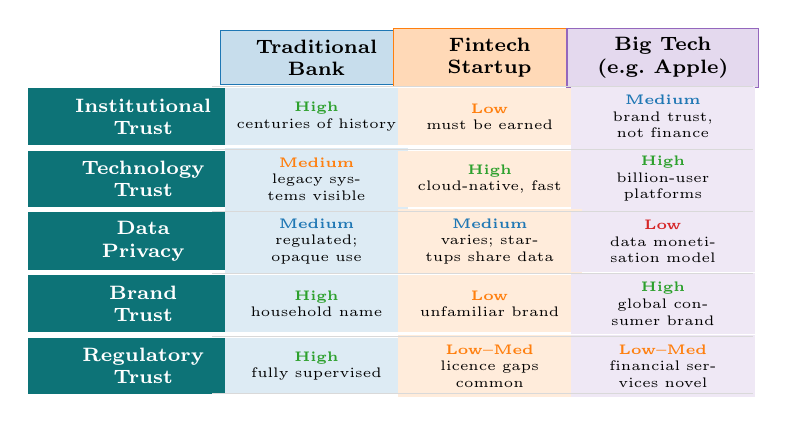
\begin{tikzpicture}[scale=0.88,
  hdr/.style={rectangle,minimum width=2.3cm,minimum height=0.65cm,
              font=\scriptsize\bfseries,text centered,text width=2.2cm},
  cell/.style={rectangle,minimum width=2.3cm,minimum height=0.72cm,
               font=\tiny,text centered,text width=2.1cm},
  dim/.style={rectangle,minimum width=2.8cm,minimum height=0.72cm,
              font=\scriptsize\bfseries,text=white,text centered,text width=2.7cm,
              fill=mlteal}
]

% ---- Column headers ----------------------------------------
\node[hdr,fill=mlblue!25,draw=mlblue]   at (3.0, 0)   {Traditional\\Bank};
\node[hdr,fill=mlorange!30,draw=mlorange] at (5.5, 0) {Fintech\\Startup};
\node[hdr,fill=mlpurple!25,draw=mlpurple] at (8.0, 0) {Big Tech\\(e.g.\ Apple)};

% ---- Row 1: Institutional trust ----------------------------
\node[dim] at (0.5,-0.85) {Institutional\\Trust};
\node[cell,fill=mlblue!15]   at (3.0,-0.85) {\textcolor{mlgreen}{\textbf{High}}\\centuries of history};
\node[cell,fill=mlorange!15] at (5.5,-0.85) {\textcolor{mlorange}{\textbf{Low}}\\must be earned};
\node[cell,fill=mlpurple!15] at (8.0,-0.85) {\textcolor{mlblue}{\textbf{Medium}}\\brand trust, not finance};

% ---- Row 2: Technology trust --------------------------------
\node[dim] at (0.5,-1.75) {Technology\\Trust};
\node[cell,fill=mlblue!15]   at (3.0,-1.75) {\textcolor{mlorange}{\textbf{Medium}}\\legacy systems visible};
\node[cell,fill=mlorange!15] at (5.5,-1.75) {\textcolor{mlgreen}{\textbf{High}}\\cloud-native, fast};
\node[cell,fill=mlpurple!15] at (8.0,-1.75) {\textcolor{mlgreen}{\textbf{High}}\\billion-user platforms};

% ---- Row 3: Data privacy ------------------------------------
\node[dim] at (0.5,-2.65) {Data\\Privacy};
\node[cell,fill=mlblue!15]   at (3.0,-2.65) {\textcolor{mlblue}{\textbf{Medium}}\\regulated; opaque use};
\node[cell,fill=mlorange!15] at (5.5,-2.65) {\textcolor{mlblue}{\textbf{Medium}}\\varies; startups share data};
\node[cell,fill=mlpurple!15] at (8.0,-2.65) {\textcolor{mlred}{\textbf{Low}}\\data monetisation model};

% ---- Row 4: Brand trust ------------------------------------
\node[dim] at (0.5,-3.55) {Brand\\Trust};
\node[cell,fill=mlblue!15]   at (3.0,-3.55) {\textcolor{mlgreen}{\textbf{High}}\\household name};
\node[cell,fill=mlorange!15] at (5.5,-3.55) {\textcolor{mlorange}{\textbf{Low}}\\unfamiliar brand};
\node[cell,fill=mlpurple!15] at (8.0,-3.55) {\textcolor{mlgreen}{\textbf{High}}\\global consumer brand};

% ---- Row 5: Regulatory trust --------------------------------
\node[dim] at (0.5,-4.45) {Regulatory\\Trust};
\node[cell,fill=mlblue!15]   at (3.0,-4.45) {\textcolor{mlgreen}{\textbf{High}}\\fully supervised};
\node[cell,fill=mlorange!15] at (5.5,-4.45) {\textcolor{mlorange}{\textbf{Low--Med}}\\licence gaps common};
\node[cell,fill=mlpurple!15] at (8.0,-4.45) {\textcolor{mlorange}{\textbf{Low--Med}}\\financial services novel};

% Horizontal grid lines
\foreach \y in {-0.42,-1.32,-2.22,-3.12,-4.02,-4.85}
  \draw[mlgray!30,thin] (1.5,\y) -- (9.3,\y);

\end{tikzpicture}
\end{center}
\bottomnote{Trust is multi-dimensional. Fintechs that partner with licensed banks can borrow institutional and regulatory trust while contributing technology trust.}
\end{frame}

% ============================================================
%  FRAME 5 -- HOW: Choice architecture diagram (TikZ)
% ============================================================
\begin{frame}{How Behavioural Design Shapes Financial Decisions}
\begin{center}
\begin{tikzpicture}[scale=0.84,
  tool/.style={rectangle,rounded corners=5pt,minimum width=2.4cm,
               minimum height=0.9cm,font=\scriptsize\bfseries,
               text centered,text width=2.3cm},
  out/.style={rectangle,rounded corners=5pt,minimum width=2.6cm,
              minimum height=0.9cm,font=\scriptsize\bfseries,
              text centered,text width=2.5cm},
  arr/.style={-{Stealth[length=5pt]},thick}
]

% ---- Title row: "Choice Architecture" box ------------------
\node[rectangle,rounded corners=5pt,fill=mlteal,text=white,
      minimum width=4.5cm,minimum height=0.75cm,
      font=\small\bfseries] (ca) at (0,2.0) {Choice Architecture};

% ---- Four tool boxes (column 1) ----------------------------
\node[tool,fill=mlblue!25,draw=mlblue]    (def) at (-3.8, 0.6) {Defaults};
\node[tool,fill=mlorange!25,draw=mlorange] (fra) at (-3.8,-0.5) {Framing};
\node[tool,fill=mlgreen!25,draw=mlgreen]  (soc) at (-3.8,-1.6) {Social Proof};
\node[tool,fill=mlpurple!25,draw=mlpurple](sim) at (-3.8,-2.7) {Simplification};

% Arrows from CA down to tools
\draw[arr,mlteal] (ca.south west) -- (def.north);
\draw[arr,mlteal] (ca.south)      -- (fra.north);
\draw[arr,mlteal] (ca.south)      -- (soc.north);
\draw[arr,mlteal] (ca.south east) -- (sim.north);

% ---- Sub-labels under tools --------------------------------
\node[font=\tiny,text=mlblue,   text width=2.3cm,align=center] at (-3.8, 0.0)
  {Pre-set saving rates,\\opt-out pension enrolment};
\node[font=\tiny,text=mlorange, text width=2.3cm,align=center] at (-3.8,-1.1)
  {Loss framing:\\``Save \$50 more/month''};
\node[font=\tiny,text=mlgreen,  text width=2.3cm,align=center] at (-3.8,-2.2)
  {``89\% of users\\round up purchases''};
\node[font=\tiny,text=mlpurple, text width=2.3cm,align=center] at (-3.8,-3.3)
  {One-tap payment,\\progress bars};

% ---- Ethical filter box (centre) ---------------------------
\node[rectangle,rounded corners=6pt,fill=mlgreen!15,draw=mlgreen,
      thick,minimum width=2.4cm,minimum height=3.8cm,
      font=\scriptsize\bfseries,text=mlgreen,
      text centered,text width=2.2cm] (eth) at (0.0,-1.1)
  {Ethical\\Filter\\[6pt]
   \tiny Transparent?\\
   \tiny Reversible?\\
   \tiny User benefit?};

\draw[arr,mlgreen!70] (-2.4, 0.6) -- (eth.west |- def);
\draw[arr,mlgreen!70] (-2.4,-0.5) -- (eth.west |- fra);
\draw[arr,mlgreen!70] (-2.4,-1.6) -- (eth.west |- soc);
\draw[arr,mlgreen!70] (-2.4,-2.7) -- (eth.west |- sim);

% ---- User Behaviour outcomes (column 3) --------------------
\node[out,fill=mlgreen!30,draw=mlgreen] (sav) at (3.8, 0.3)
  {Higher\\Savings Rate};
\node[out,fill=mlblue!25,draw=mlblue]  (ins) at (3.8,-1.1)
  {Better\\Insurance\\Take-up};
\node[out,fill=mlred!20,draw=mlred]    (drk) at (3.8,-2.5)
  {Dark Pattern\\(if filter fails)};

\draw[arr,mlgreen] (eth.east) -- (sav.west);
\draw[arr,mlblue]  (eth.east) -- (ins.west);
\draw[arr,mlred,dashed] (eth.east) -- (drk.west);

% Dark pattern label
\node[font=\tiny\itshape,text=mlred,text width=2.8cm,align=center]
  at (3.8,-3.15) {Hidden fees, deceptive\\opt-out flows};

\end{tikzpicture}
\end{center}
\bottomnote{Choice architecture is not inherently good or bad. The ethical filter is what distinguishes fintech that empowers users from fintech that exploits them.}
\end{frame}

% ============================================================
%  FRAME 6 -- RISK: TikZ comic (dark pattern caught by colleague)
% ============================================================
\begin{frame}{When Design Becomes Manipulation: Dark Patterns}
\begin{columns}[T]
\begin{column}{0.52\textwidth}
\vspace{0.2em}
\begin{center}
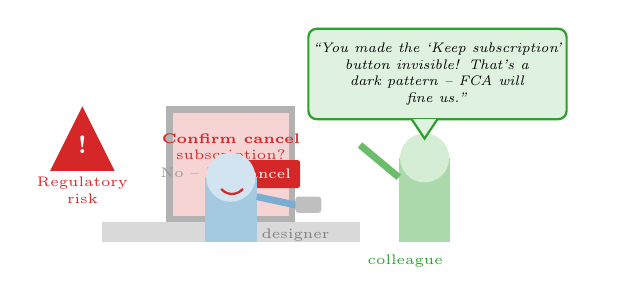
\begin{tikzpicture}[scale=0.82]

  % ---- Designer at desk ------------------------------------
  % Desk
  \fill[mlgray!30] (-2.0,-0.6) rectangle (2.0,-0.3);
  % Monitor
  \fill[mlgray!60] (-1.0,-0.3) rectangle (1.0,1.5);
  \fill[mlred!20]  (-0.9,-0.2) rectangle (0.9,1.4);
  % Screen text (dark pattern)
  \node[font=\tiny,text=mlred,align=center] at (0.0,0.85)
    {\textbf{Confirm cancel}\\subscription?};
  \node[font=\tiny,text=mlred] at (-0.45,0.45) {\textcolor{mlgray!80}{\tiny No -- keep}};
  \node[font=\tiny,text=white,fill=mlred,rounded corners=1pt]
    at (0.5,0.45) {Cancel};
  % Monitor stand
  \fill[mlgray!50] (-0.15,-0.6) rectangle (0.15,-0.3);
  % Designer body
  \fill[mlblue!40] (-0.4,-0.6) rectangle (0.4,0.4);
  % Head
  \fill[mlblue!20] (0.0,0.4) circle (0.38);
  % Evil grin -- arc
  \draw[mlred,thick] (-0.15,0.22) arc(220:320:0.22);
  % Arm to mouse
  \draw[mlblue!60,line width=2.5pt] (0.4,0.1) -- (1.1,-0.05);
  \fill[mlgray!50,rounded corners=1pt] (1.0,-0.15) rectangle (1.4,0.1);
  \node[font=\tiny,text=mlgray] at (1.0,-0.5) {designer};

  % ---- Colleague bursting in (right) -------------------------
  % Body
  \fill[mlgreen!40] (2.6,-0.6) rectangle (3.4,0.7);
  % Head
  \fill[mlgreen!20] (3.0,0.7) circle (0.38);
  % Raised hand
  \draw[mlgreen!70,line width=2.5pt] (2.6,0.4) -- (2.0,0.9);
  \node[font=\tiny,text=mlgreen] at (2.7,-0.9) {colleague};

  % ---- Colleague speech bubble --------------------------------
  \fill[mlgreen!15,rounded corners=3pt] (1.2,1.3) rectangle (5.2,2.7);
  \draw[mlgreen,thick,rounded corners=3pt] (1.2,1.3) rectangle (5.2,2.7);
  \fill[mlgreen!15] (2.8,1.3) -- (3.0,1.0) -- (3.2,1.3) -- cycle;
  \draw[mlgreen,thick] (2.8,1.3) -- (3.0,1.0) -- (3.2,1.3);
  \node[font=\tiny,text width=3.6cm,align=center] at (3.2,2.0)
    {\textit{``You made the `Keep subscription'}\\
     \textit{button invisible! That's a}\\
     \textit{dark pattern -- FCA will}\\
     \textit{fine us.''}};

  % ---- Warning triangle (bottom left) ------------------------
  \fill[mlred] (-2.8,0.5) -- (-2.3,1.5) -- (-1.8,0.5) -- cycle;
  \node[font=\small\bfseries,text=white] at (-2.3,0.9) {!};
  \node[font=\tiny,text=mlred,align=center] at (-2.3,0.2)
    {Regulatory\\risk};

\end{tikzpicture}
\end{center}
\end{column}
\begin{column}{0.44\textwidth}
\vspace{0.2em}
\begin{alertblock}{Dark Pattern Types in Fintech}
\scriptsize
\textbf{Roach Motel:} Easy to sign up, very hard to cancel.\\[2pt]
\textbf{Confirmshaming:} ``No thanks, I don't want to save money.''\\[2pt]
\textbf{Hidden Costs:} Fees revealed only at final checkout.\\[2pt]
\textbf{Misdirection:} Highlight the option you want the user to \emph{avoid}.
\end{alertblock}
\vspace{0.2em}
\begin{block}{Regulatory Response}
\scriptsize
FCA (UK) 2023 Consumer Duty requires firms to prove good outcomes for customers.\\[2pt]
CFPB (US) targets ``junk fees'' and subscription traps.\\[2pt]
EU Digital Services Act covers deceptive interfaces.
\end{block}
\end{column}
\end{columns}
\bottomnote{The line between persuasion and manipulation is a regulatory frontier. Fintech designers now face the same scrutiny as pharmaceutical advertisers.}
\end{frame}

% ============================================================
%  FRAME 7 -- WHERE: pgfplots bar chart (financial inclusion gap)
% ============================================================
\begin{frame}{Where Is the Gap? Financial Inclusion by Region}
\vspace{0.05em}
\begin{center}
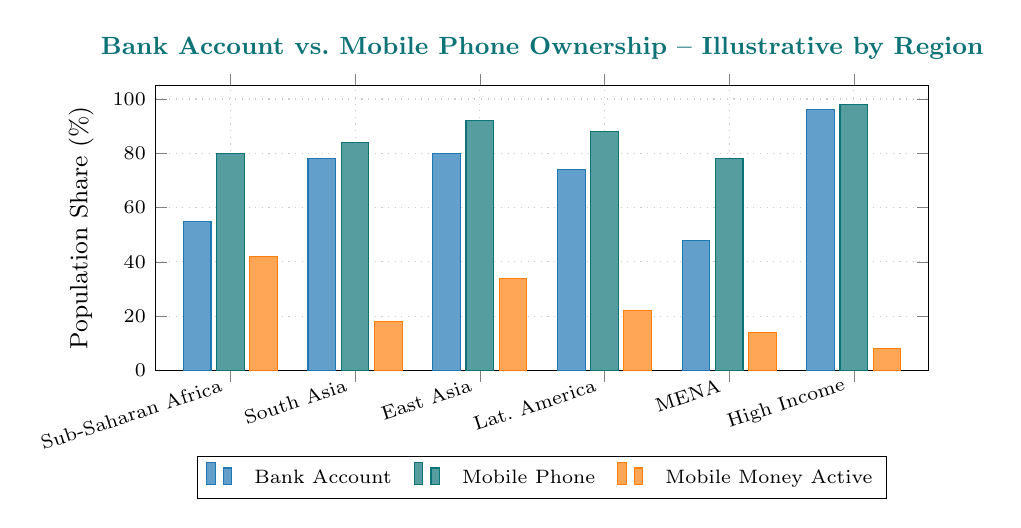
\begin{tikzpicture}
\begin{axis}[
  width=11.4cm, height=5.2cm,
  ybar=2pt,
  bar width=10pt,
  enlarge x limits=0.12,
  ylabel={\small Population Share (\%)},
  ylabel style={font=\small},
  symbolic x coords={Sub-Saharan Africa, South Asia, East Asia, Lat.\ America, MENA, High Income},
  xtick=data,
  xticklabel style={font=\scriptsize, rotate=18, anchor=east},
  ymin=0, ymax=105,
  ytick={0,20,40,60,80,100},
  yticklabel style={font=\scriptsize},
  legend style={font=\scriptsize, at={(0.5,-0.30)}, anchor=north,
                legend columns=3, column sep=6pt},
  legend cell align=left,
  grid=major,
  grid style={dotted,mlgray!40},
  title={\small\bfseries\textcolor{mlteal}{Bank Account vs.\ Mobile Phone Ownership -- Illustrative by Region}},
  title style={font=\small},
  clip=false,
]

% Bank account ownership (%)
\addplot[fill=mlblue!70,draw=mlblue] coordinates {
  (Sub-Saharan Africa,  55)
  (South Asia,          78)
  (East Asia,           80)
  (Lat.\ America,       74)
  (MENA,                48)
  (High Income,         96)
};

% Mobile phone ownership (%)
\addplot[fill=mlteal!70,draw=mlteal] coordinates {
  (Sub-Saharan Africa,  80)
  (South Asia,          84)
  (East Asia,           92)
  (Lat.\ America,       88)
  (MENA,                78)
  (High Income,         98)
};

% Mobile money active users (%) -- subset
\addplot[fill=mlorange!70,draw=mlorange] coordinates {
  (Sub-Saharan Africa,  42)
  (South Asia,          18)
  (East Asia,           34)
  (Lat.\ America,       22)
  (MENA,                14)
  (High Income,          8)
};

\legend{Bank Account, Mobile Phone, Mobile Money Active}
\end{axis}
\end{tikzpicture}
\end{center}
\vspace{-0.5em}
{\tiny\textcolor{mlgray}{Illustrative figures based on World Bank Global Findex 2021 and GSMA State of Mobile 2023 trends. Mobile money active = at least one transaction per 90 days.}}
\bottomnote{The ``mobile gap'' (phones minus bank accounts) is largest in Sub-Saharan Africa and MENA -- and represents the biggest addressable market for mobile-first fintech.}
\end{frame}

% ============================================================
%  FRAME 8 -- IMPACT: Quadrant diagram (Inclusion vs. Protection)
% ============================================================
\begin{frame}{The Ecosystem Trade-off: Inclusion vs.\ Protection}
\vspace{0.1em}
\begin{center}
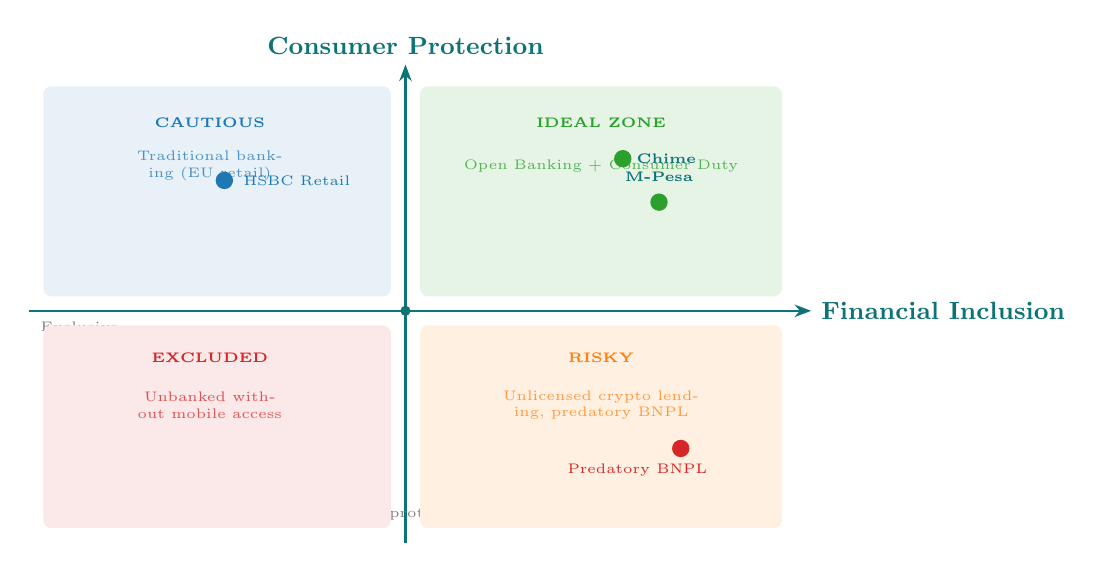
\begin{tikzpicture}[scale=0.92]

  % ---- Axes --------------------------------------------------
  \draw[-{Stealth[length=6pt]},mlteal,thick] (-5.2,0) -- (5.6,0)
    node[right,font=\small\bfseries,text=mlteal] {Financial Inclusion};
  \draw[-{Stealth[length=6pt]},mlteal,thick] (0,-3.2) -- (0,3.4)
    node[above,font=\small\bfseries,text=mlteal] {Consumer Protection};

  % Axis labels (negative ends)
  \node[font=\tiny,text=mlgray] at (-4.5,-0.22) {Exclusive};
  \node[font=\tiny,text=mlgray] at ( 0.15,-2.8)  {Unprotected};

  % ---- Quadrant labels --------------------------------------
  % Q1: High inclusion, High protection (ideal)
  \fill[mlgreen!12,rounded corners=3pt] (0.2,0.2) rectangle (5.2,3.1);
  \node[font=\tiny\bfseries,text=mlgreen,align=center] at (2.7,2.6)
    {IDEAL ZONE};
  \node[font=\tiny,text=mlgreen!80,align=center,text width=3.5cm] at (2.7,2.0)
    {Open Banking + Consumer Duty};

  % Q2: Low inclusion, High protection (cautious)
  \fill[mlblue!10,rounded corners=3pt] (-5.0,0.2) rectangle (-0.2,3.1);
  \node[font=\tiny\bfseries,text=mlblue,align=center] at (-2.7,2.6)
    {CAUTIOUS};
  \node[font=\tiny,text=mlblue!80,align=center,text width=3.3cm] at (-2.7,2.0)
    {Traditional banking (EU retail)};

  % Q3: Low inclusion, Low protection (excluded)
  \fill[mlred!10,rounded corners=3pt] (-5.0,-3.0) rectangle (-0.2,-0.2);
  \node[font=\tiny\bfseries,text=mlred,align=center] at (-2.7,-0.65)
    {EXCLUDED};
  \node[font=\tiny,text=mlred!80,align=center,text width=3.3cm] at (-2.7,-1.3)
    {Unbanked without mobile access};

  % Q4: High inclusion, Low protection (risky)
  \fill[mlorange!12,rounded corners=3pt] (0.2,-3.0) rectangle (5.2,-0.2);
  \node[font=\tiny\bfseries,text=mlorange,align=center] at (2.7,-0.65)
    {RISKY};
  \node[font=\tiny,text=mlorange!80,align=center,text width=3.5cm] at (2.7,-1.3)
    {Unlicensed crypto lending, predatory BNPL};

  % ---- Example dots -----------------------------------------
  % M-Pesa
  \fill[mlgreen] (3.5,1.5) circle (0.12);
  \node[font=\tiny\bfseries,text=mlteal] at (3.5,1.85) {M-Pesa};

  % Chime
  \fill[mlgreen] (3.0,2.1) circle (0.12);
  \node[font=\tiny\bfseries,text=mlteal] at (3.6,2.1) {Chime};

  % Traditional UK bank
  \fill[mlblue] (-2.5,1.8) circle (0.12);
  \node[font=\tiny,text=mlblue] at (-1.5,1.8) {HSBC Retail};

  % Predatory BNPL
  \fill[mlred] (3.8,-1.9) circle (0.12);
  \node[font=\tiny,text=mlred] at (3.2,-2.2) {Predatory BNPL};

  % Origin crosshair
  \fill[mlteal] (0,0) circle (0.07);

\end{tikzpicture}
\end{center}
\bottomnote{Policy goal: move the ecosystem toward the top-right quadrant -- high inclusion AND high protection. The two are not inherently in tension.}
\end{frame}

% ============================================================
%  FRAME 9 -- SO WHAT: Evaluation checklist with TikZ checkmarks
% ============================================================
\begin{frame}{So What? Five Questions to Evaluate Any Fintech Ecosystem}

\vspace{0.3em}
\begin{columns}[T]
\begin{column}{0.62\textwidth}

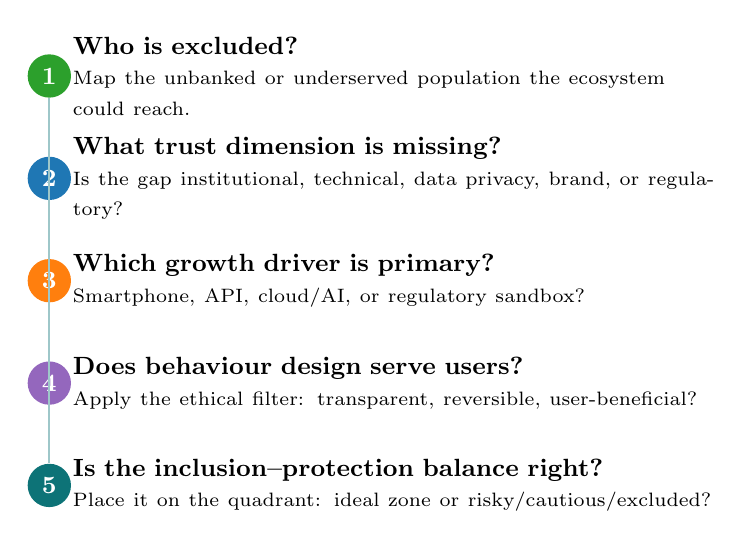
\begin{tikzpicture}[
  chk/.style={circle,minimum size=0.55cm,font=\small\bfseries,
              inner sep=0pt,text=white},
  lbl/.style={font=\small,text width=8.2cm,align=left}
]

% ---- Row 1 --------------------------------------------------
\node[chk,fill=mlgreen]  (c1) at (0, 0)   {1};
\node[lbl] at (4.4, 0)
  {\textbf{Who is excluded?}\\
   {\scriptsize Map the unbanked or underserved population the ecosystem could reach.}};

% ---- Row 2 --------------------------------------------------
\node[chk,fill=mlblue]   (c2) at (0,-1.3) {2};
\node[lbl] at (4.4,-1.3)
  {\textbf{What trust dimension is missing?}\\
   {\scriptsize Is the gap institutional, technical, data privacy, brand, or regulatory?}};

% ---- Row 3 --------------------------------------------------
\node[chk,fill=mlorange] (c3) at (0,-2.6) {3};
\node[lbl] at (4.4,-2.6)
  {\textbf{Which growth driver is primary?}\\
   {\scriptsize Smartphone, API, cloud/AI, or regulatory sandbox?}};

% ---- Row 4 --------------------------------------------------
\node[chk,fill=mlpurple] (c4) at (0,-3.9) {4};
\node[lbl] at (4.4,-3.9)
  {\textbf{Does behaviour design serve users?}\\
   {\scriptsize Apply the ethical filter: transparent, reversible, user-beneficial?}};

% ---- Row 5 --------------------------------------------------
\node[chk,fill=mlteal]   (c5) at (0,-5.2) {5};
\node[lbl] at (4.4,-5.2)
  {\textbf{Is the inclusion--protection balance right?}\\
   {\scriptsize Place it on the quadrant: ideal zone or risky/cautious/excluded?}};

% Vertical connector line
\draw[mlteal!40,thick] (0,-0.28) -- (0,-4.92);

\end{tikzpicture}

\end{column}
\begin{column}{0.34\textwidth}
\vspace{0.2em}
\begin{block}{When to Use This}
\scriptsize
\begin{itemize}
  \item Evaluating a VC pitch
  \item Writing a policy brief
  \item Assessing a job offer at a fintech
  \item Completing the Day-5 Workshop C exercise
\end{itemize}
\end{block}
\vspace{0.2em}
\begin{exampleblock}{Worked Example}
\scriptsize
\textbf{M-Pesa Kenya (2007)}\\
Excluded: rural unbanked\\
Trust gap: institutional\\
Driver: smartphone\\
Behaviour: simple USSD defaults\\
Quadrant: moves toward ideal
\end{exampleblock}
\end{column}
\end{columns}

\bottomnote{These five questions distil L01--L02 into a reusable diagnostic. You will return to them in every lecture that follows.}
\end{frame}

% ============================================================
%  FRAME 10 -- ACT: Activity frame (ecosystem evaluation exercise)
% ============================================================
\begin{frame}{Act: Apply the Ecosystem Evaluation to a Fintech You Use}

\begin{columns}[T]
\begin{column}{0.56\textwidth}
\begin{block}{Your Task (15 Minutes)}
\scriptsize
Choose \textbf{one fintech product} you use regularly. Work through the five-question framework:
\begin{enumerate}\scriptsize
  \item \textbf{Excluded population:} Who was this built for? Who does it still fail to reach?
  \item \textbf{Trust gap:} Which trust dimension did it have to overcome, and how?
  \item \textbf{Growth driver:} Which of the four engines powers it?
  \item \textbf{Behavioural design:} Find one nudge. Benevolent or dark?
  \item \textbf{Quadrant placement:} Draw it on the 2x2. Ideal zone? How to get there?
\end{enumerate}
\end{block}
\end{column}
\begin{column}{0.40\textwidth}
\begin{exampleblock}{Reflection Prompts}
\scriptsize
\begin{itemize}
  \item As the \textbf{regulator}: what would you require to change?
  \item As the \textbf{founder}: what would you do to serve the excluded?
  \item Is this product \textbf{creating} or \textbf{capturing} value?
\end{itemize}
\end{exampleblock}
\begin{alertblock}{Next Lecture -- L03}
\scriptsize \textbf{Payments \& Digital Currencies}\\
From cash to crypto: how value moves in a digital ecosystem.\\
\textit{Prepare: read your payment app's fee schedule.}
\end{alertblock}
\end{column}
\end{columns}

\bottomnote{The ecosystem is not fixed: products move on the quadrant as regulation tightens, trust grows, or technology improves. Your job is to track the direction of travel.}
\end{frame}

% ============================================================
\end{document}
% ============================================================
